\documentclass[dvipsnames,table]{beamer}
\usepackage{pgf, pgffor}
\usepackage{lstlinebgrd}
\usepackage{subcaption}
\usepackage{color}

\makeatletter
\newcount\bt@rangea
\newcount\bt@rangeb


% Code copied from http://tex.stackexchange.com/questions/8851/how-can-i-highlight-some-lines-from-source-code.
% I don't understand it.  But it seems to do what I want it to do.

%%%%%%%%%%%%%%%%%%%%%%%%%%%%%%%%%%%%%%%%%%%%%%%%%%%%%%%%%%%%%%%%%%%%%%%%%%%%%%
%
% \btIfInRange{number}{range list}{TRUE}{FALSE}
%
% Test in int number <number> is element of a (comma separated) list of ranges
% (such as: {1,3-5,7,10-12,14}) and processes <TRUE> or <FALSE> respectively
\newcommand\btIfInRange[2]{%
    \global\let\bt@inrange\@secondoftwo%
    \edef\bt@rangelist{#2}%
    \foreach \range in \bt@rangelist {%
        \afterassignment\bt@getrangeb%
        \bt@rangea=0\range\relax%
        \pgfmathtruncatemacro\result{ ( #1 >= \bt@rangea) && (#1 <= \bt@rangeb) }%
        \ifnum\result=1\relax%
            \breakforeach%
            \global\let\bt@inrange\@firstoftwo%
        \fi%
    }%
    \bt@inrange%
}
\newcommand\bt@getrangeb{%
    \@ifnextchar\relax%
        {\bt@rangeb=\bt@rangea}%
        {\@getrangeb}%
}
\def\@getrangeb-#1\relax{%
    \ifx\relax#1\relax%
        \bt@rangeb=100000%   \maxdimen is too large for pgfmath
    \else%
        \bt@rangeb=#1\relax%
    \fi%
}

%%%%%%%%%%%%%%%%%%%%%%%%%%%%%%%%%%%%%%%%%%%%%%%%%%%%%%%%%%%%%%%%%%%%%%%%%%%%%%
%
% \btLstHL<overlay spec>{range list}
%
% TODO BUG: \btLstHL commands can not yet be accumulated if more than one overlay spec match.
% 
\newcommand<>{\btLstHL}[1]{%
  \only#2{\btIfInRange{\value{lstnumber}}{#1}{\color{orange!30}\def\lst@linebgrdcmd{\color@block}}{\def\lst@linebgrdcmd####1####2####3{}}}%
}%
\makeatother

%%%%%%%%%%%%%%%%%%%%%%%%%%%%%%%%%%%%%%%%%%%%%%%%%%%%%%%%%%%%%%%%%%%%%%%%%%%%%%

\usepackage{color}
\definecolor{lightgray}{rgb}{.9,.9,.9}
\definecolor{darkgray}{rgb}{.4,.4,.4}
\definecolor{purple}{rgb}{0.65, 0.12, 0.82}


% Code copied from http://tex.stackexchange.com/questions/89574/language-option-supported-in-listings
\lstdefinelanguage{JavaScript}{
  keywords={typeof, new, true, false, catch, function, return, null, catch, switch, var, if, in, while, do, else, case, break},
  keywordstyle=\color{blue}\bfseries,
  ndkeywords={class, export, boolean, throw, implements, import, this},
  ndkeywordstyle=\color{darkgray}\bfseries,
  identifierstyle=\color{black},
  sensitive=false,
  comment=[l]{//},
  morecomment=[s]{/*}{*/},
  commentstyle=\color{purple}\ttfamily,
  stringstyle=\color{red}\ttfamily,
  morestring=[b]',
  morestring=[b]"
}


\lstdefinestyle{small1XML}{language=XML,backgroundcolor=\color{lightgray},basicstyle=\ttfamily\small}
\lstdefinestyle{small2XML}{language=XML,backgroundcolor=\color{lightgray},basicstyle=\ttfamily\scriptsize}
\lstdefinestyle{small3XML}{language=XML,backgroundcolor=\color{lightgray},basicstyle=\ttfamily\tiny}
\lstdefinestyle{small1HTML}{language=HTML,backgroundcolor=\color{lightgray},basicstyle=\ttfamily\small}
\lstdefinestyle{small2HTML}{language=HTML,backgroundcolor=\color{lightgray},basicstyle=\ttfamily\scriptsize}
\lstdefinestyle{small3HTML}{language=HTML,backgroundcolor=\color{lightgray},basicstyle=\ttfamily\tiny}
\lstdefinestyle{small2js}{language=JavaScript,backgroundcolor=\color{lightgray},basicstyle=\ttfamily\scriptsize}

\mode<presentation>
{\usetheme{iSEC} % or use any builtin beamer theme
\setbeamercovered{transparent}}

% Uncomment these to use times instead
%\usepackage{times}

% Or whatever. Note that the encoding and the font should match. If T1
% does not look nice, try deleting the line with the fontenc.

\title[The SVG Security Model]{The SVG Security Model}
\subtitle{When an image isn't just an image}
\author[Rennie deGraaf]{Rennie deGraaf}
\institute[iSEC Partners]{\Large iSEC Partners}
\date[Amazon Friday Learning Series]{6 February 2015}
\titlegraphic{
\includegraphics[height=1.5cm]{images/Amazon_logo}}
\logo{
\includegraphics[height=0.8cm]{images/iseclogo.pdf}}

\subject{Application Security}
% This is only inserted into the PDF information catalog. Can be left
% out. 

% Uncomment this, if you want the table of contents to pop up at
% the beginning of each subsection:
%\AtBeginSubsection[]
%{\begin{frame}<beamer>{Outline}
%    \tableofcontents[currentsection,currentsubsection]
%  \end{frame}
%}

% If you wish to uncover everything in a step-wise fashion, uncomment
% the following command: 

%\beamerdefaultoverlayspecification{<+->}

% Change the level of bulleting on the ToC page
\setcounter{tocdepth}{2}

\begin{document}

\begin{frame}
  \titlepage
\end{frame}

\begin{frame}{Outline}
  \tableofcontents
  % You might wish to add the option [pausesections]
\end{frame}


\section{Review of web security}

\begin{frame}[fragile]{Web Security}
  \begin{itemize}
    \item A page can request resources from any source, but there are restrictions on how those resources can interact.
    \item Web security is a confusing mix of rules that apply to different things, work-arounds to those rules, and mitigations against attacks permitted by those rules.
    \item Most important rule: Same-Origin Policy
    \item Most important mitigation: Content Security Policy
  \end{itemize}
\end{frame}

\subsection{Same-Origin Policy}

\begin{frame}[fragile]{Same-Origin Policy}
  \begin{itemize}
    \item An \emph{origin} is a (protocol, host, port) tuple.
    \item Unless you're Internet Explorer, which ignores the port.
    \item Scripts running inside a page from one origin can only interact with resources from the same origin.
    \item \url{http://www.example.com/somedir/page.html} has the same origin as \url{http://www.example.com/otherdir/doc.html}, but not the same origin as \url{https://www.example.com/somedir/page2.html} or \url{http://en.example.com}.
    \item The origin of a script is the origin of the page that loaded it, not the origin from which the script was loaded.
    \item This restriction can be relaxed in various ways.
    \item Cookies, Flash, \texttt{file:} URIs, and some other things have different rules.
  \end{itemize}
\end{frame}

\subsection{Content Security Policy}

\begin{frame}[fragile]{Content Security Policy}{An introduction}
  \begin{itemize}
    %\item Exploit mitigation system. 
    \item Policies restrict the allowed sources for scripts, styles, images, etc.  Resources may only come from white-listed origins.
    \item Blocks mixed content: \texttt{eval}, in-line scripts and styles, \texttt{data:} URIs, etc.
    \item Can be used to restrict content to \texttt{https:} URIs.
    \item Sent by the server in \texttt{Content-Security-Policy} headers; enforced by the browser.
    \item First standardized in 2012.
    \item Firefox and Chrome have supported it for a while.  The latest Internet Explorer technical preview build also supports it.
  \end{itemize}
\end{frame}

\begin{frame}[fragile]{Content Security Policy}{Directives}
  \begin{itemize}
    \item A policy is built from from directives that control the allowed sources for specific types of content:
  \end{itemize}
  \begin{description}
    \item[script-src] Scripts, XSLT
    \item[style-src] Styles
    \item[img-src] Images, including \texttt{img} tags and various CSS properties
    \item[frame-src] Documents or data loaded from \texttt{frame} or \texttt{iframe} tags
    \item[object-src] Documents, data, or plugins from \texttt{object}, \texttt{embed}, or \texttt{applet} tags
    \item[media-src] Audio and video content, such as \texttt{video} and \texttt{audio} tags
    \item[font-src] Fonts
    \item[connect-src] \texttt{XMLHttpRequest}, WebSockets, etc.
    \item[default-src] Defaults for any directive that isn't specified
  \end{description}
\end{frame}

\begin{frame}[fragile]{Content Security Policy}{Source lists}
  \begin{itemize}
    \item Each directive must have a source list.  Sources\footnote{A \emph{source} is a scheme-host-port tuple, but differs from the document \emph{origin} under some circumstances.} can be
  \end{itemize}
  \begin{description}
    \item['none'] Content covered by the directive must not be allowed from any source.
    \item['self'] The source of the document to which CSP applies.
    \item[<host>] A host name.  Some wildcards are allowed.  A URI scheme and port number may also be supplied.
    \item[<scheme>] A URI scheme.
  \end{description}
  \begin{itemize}
    \item If a document attempts to load a resource covered by CSP, and the resource's source is not in the source list for the applicable directive, then the user agent must not load the resource.
  \end{itemize}
\end{frame}

\begin{frame}[fragile]{Content Security Policy}{An example}
  \setbeamercovered{transparent}
  \texttt{Content-Security-Policy: \uncover<1,6>{default-src 'none';} \uncover<2,6>{style-src 'self';} \uncover<3,6>{script-src 'self' https:;} \uncover<4,6>{img-src 'self' data: *.svg.test;} \uncover<5,6>{object-src 'self' http://images.svg.test; frame-src 'self' http://images.svg.test;}}
  \setbeamercovered{opaque}
  \begin{itemize}[<+->]
    \item Defaults to not allowing any content from any source.
    \item Styles are only allowed from external files at the same source as the document.
    \item Scripts are only allowed from external files at the same source, and from other sources over HTTPS.
    \item Static images are allowed from from files at the same source, \texttt{data:} URIs, and from files at \texttt{*.svg.test}.
    \item Objects and frames are allowed from the same source and from \texttt{http://images.svg.test}.
    \item Media, fonts, and connections are not allowed on any source.
  \end{itemize}
\end{frame}

\begin{frame}[fragile]{Content Security Policy}{More things to know}
  \begin{itemize}
    \item If more than one CSP applies to a document, then all policies must be applied independently.
    \item \emph{Only} the CSP served with an embedded document applies to that document; any CSPs that apply to the parent context are ignored.
    \item There is a report-only mode for debugging.
    \item There are ways to allow in-line scripts and stylesheets, and to allow \texttt{eval} in scripts.  Don't use them.
  \end{itemize}
\end{frame}

\begin{frame}[fragile]{Content Security Policy}{Why you should use it}
  \begin{itemize}
    \item Exploit mitigation.  Think ASLR+DEP for web apps.
    \item It's hard to get XSS if the browser will only execute scripts from white-listed static documents and \texttt{eval} is banned globally.
    \item A lot of web frameworks like to mix content, scripts, and styles, so get started on separating them as soon as possible.
    \item More information: \url{http://content-security-policy.com/}, \url{https://www.isecpartners.com/media/106598/csp_best_practices.pdf}
    %\item It also applies to SVG!
  \end{itemize}
\end{frame}


\section{A brief introduction to SVG}

\subsection{What is SVG?}

\begin{frame}[fragile]{What is SVG?}
  \begin{itemize}
    \item \textbf{S}calable \textbf{V}ector \textbf{G}raphics
    \item XML-based
    \item W3C (\url{http://www.w3.org/TR/SVG/})
    \item Development started in 1999
    \item Current version is 1.1, published in 2011
    \item Version 2.0 is in development
    \item First browser with native support was Konqueror in 2004; 
    \item IE was the last major browser to add native SVG support (IE9, in 2011)
  \end{itemize}
\end{frame}

\begin{frame}[fragile]{Disclaimer}{I am not an artist.}
  \hfill
\includegraphics[height=5cm]{includes/dammitjim}\hspace*{\fill}
\end{frame}

\begin{frame}[fragile]{A simple example}{As rendered}
  \hfill
\includegraphics[height=2cm]{includes/circle}\hspace*{\fill}
\end{frame}

\begin{frame}[fragile]{A simple example}{Source code}
  \lstinputlisting[language=XML]{includes/circle.svg}
\end{frame}

\subsection{Using SVG with HTML}

\begin{frame}[fragile]{Embedding SVG in HTML}
  \begin{itemize}
    \item As a static image:
    \begin{itemize}
      \item \texttt{img} tag
      \item CSS resources (eg, \texttt{background-image})
    \end{itemize}
    \item As a nested document
    \begin{itemize}
      \item \texttt{object} tag
      \item \texttt{embed} tag
      \item \texttt{iframe} tag
    \end{itemize}
   \item In-line
   \item \texttt{canvas} tag
  \end{itemize}
\end{frame}

%\begin{frame}[fragile]{Embedding SVG in HTML}{Using \texttt{img} tags}
%  \lstinputlisting[style=small1HTML,linebackgroundcolor={\btLstHL<1>{5}}]{includes/svg-img.html}
%\end{frame}

%\begin{frame}[fragile]{Embedding SVG in HTML}{Using CSS resources}
%  \lstinputlisting[style=small1HTML,linebackgroundcolor={\btLstHL<1>{5}}]{includes/svg-css.html}
%\end{frame}

%\begin{frame}[fragile]{Embedding SVG in HTML}{Using \texttt{data:} URIs}
%  \lstinputlisting[style=small2HTML,breaklines=true,linebackgroundcolor={\btLstHL<1>{5-13}}]{includes/svg-data.html}
%\end{frame}

%\begin{frame}[fragile]{Embedding SVG in HTML}{Using \texttt{object} tags}
%  \lstinputlisting[style=small1HTML,linebackgroundcolor={\btLstHL<1>{5}}]{includes/svg-object.html}
%\end{frame}

%\begin{frame}[fragile]{Embedding SVG in HTML}{Using \texttt{embed} tags}
%  \lstinputlisting[style=small1HTML,linebackgroundcolor={\btLstHL<1>{5}}]{includes/svg-embed.html}
%\end{frame}

%\begin{frame}[fragile]{Embedding SVG in HTML}{Using \texttt{iframe} tags}
%  \lstinputlisting[style=small1HTML,linebackgroundcolor={\btLstHL<1>{5}}]{includes/svg-iframe.html}
%\end{frame}

%\begin{frame}[fragile]{Embedding SVG in HTML}{Using in-line SVG}
%  \lstinputlisting[style=small2HTML,breaklines=true,linebackgroundcolor={\btLstHL<1>{5-16}}]{includes/svg-inline.html}
%\end{frame}

%\begin{frame}[fragile]{Embedding SVG in HTML}{Other ways}
%  \begin{itemize}
%    \item \texttt{canvas}
%    \item Other CSS properties
%    \item I'm sure that there are more.
%  \end{itemize}
%\end{frame}

\subsection{SVG features}

\begin{frame}[fragile]{SVG with CSS}{In-line}
  \lstinputlisting[style=small1XML,linebackgroundcolor={\btLstHL<1>{8-10}}]{includes/circle-css.svg}
\end{frame}

\begin{frame}[fragile]{SVG with CSS}{External}
  \lstinputlisting[style=small1XML,linebackgroundcolor={\btLstHL<1>{3-4}}]{includes/circle-css-external.svg}
\end{frame}

\begin{frame}[fragile]{SVG with CSS}{As rendered}
\begin{figure}
\centering
\begin{subfigure}{.5\textwidth}
  \centering
  
\includegraphics[height=2cm]{includes/circle}
  \caption{Without CSS}
\end{subfigure}%
\begin{subfigure}{.5\textwidth}
  \centering
  
\includegraphics[height=2cm]{includes/circle-css}
  \caption{With CSS}
\end{subfigure}
\end{figure}
\end{frame}

\begin{frame}[fragile]{SVG with JavaScript}{In-line}
  \lstinputlisting[style=small2XML,linebackgroundcolor={\btLstHL<1>{8-13}}]{includes/circle-js.svg}
\end{frame}

\begin{frame}[fragile]{SVG with JavaScript}{External}
  \lstinputlisting[style=small1XML,linebackgroundcolor={\btLstHL<1>{9}}]{includes/circle-js-external.svg}
\end{frame}

\begin{frame}[fragile]{SVG with JavaScript}{As rendered}
\begin{figure}
\centering
\begin{subfigure}{.5\textwidth}
  \centering
  
\includegraphics[height=2cm]{includes/circle}
  \caption{Without JavaScript}
\end{subfigure}%
\begin{subfigure}{.5\textwidth}
  \centering
  
\includegraphics[height=2cm]{includes/circle-js}
  \caption{With JavaScript}
\end{subfigure}
\end{figure}
\end{frame}

\begin{frame}[fragile]{SVG with an external image}
  \lstinputlisting[style=small2XML,linebackgroundcolor={\btLstHL<1>{14}}]{includes/circle-image.svg}
\end{frame}

\begin{frame}[fragile]{SVG with an external image}{As rendered}
\begin{figure}
\centering
\begin{subfigure}{.5\textwidth}
  \centering
  
\includegraphics[height=2cm]{includes/circle}
  \caption{Normal}
\end{subfigure}%
\begin{subfigure}{.5\textwidth}
  \centering
  
\includegraphics[height=2cm]{includes/circle-image}
  \caption{With an external image}
\end{subfigure}
\end{figure}
\end{frame}

\begin{frame}[fragile]{SVG with embedded HTML}
  \lstinputlisting[style=small3XML,linebackgroundcolor={\btLstHL<1>{14-25}}]{includes/circle-foreign-html.svg}
\end{frame}

\begin{frame}[fragile]{SVG with embedded HTML}{As rendered}
\begin{figure}
\centering
\begin{subfigure}{.5\textwidth}
  \centering
  
\includegraphics[height=2cm]{includes/circle}
  \caption{Normal}
\end{subfigure}%
\begin{subfigure}{.5\textwidth}
  \centering
  
\includegraphics[height=2cm]{includes/circle-image}
  \caption{With another SVG embedded inside HTML in a \texttt{foreignObject}}
\end{subfigure}
\end{figure}
\end{frame}

\begin{frame}[fragile]{In-line SVG}
  \lstinputlisting[style=small3HTML,breaklines=true,linebackgroundcolor={\btLstHL<1>{5-16}}]{includes/svg-inline.html}
  \begin{itemize}
    \item Considered part of the document.
    \item Can load its own scripts.
    \item \texttt{xml-stylesheet} directives aren't allowed in HTML, but any stylesheets applied to the HTML document also apply to in-line SVG.
  \end{itemize}
\end{frame}

\section{Attacking SVG}
\subsection{Attack surface}

\begin{frame}[fragile]{Attack surface}
  Since SVG can do pretty much everything that HTML can do, the attack surface is very similar:
  \begin{itemize}
    \item XML attacks (Billion Laughs, etc.)
    \item DOM attacks
    \item XSS
    \item Etc.
  \end{itemize}
\end{frame}

\begin{frame}[fragile]{Billion Laughs}
  \lstinputlisting[style=small3XML,linebackgroundcolor={\btLstHL<1>{5-14,27}}]{includes/circle-lol.svg}
\end{frame}

\begin{frame}[fragile]{Billion Laughs}{Chrome}
\begin{figure}
  \centering
  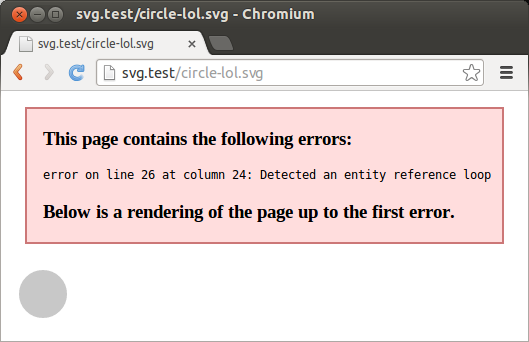
\includegraphics[height=5cm]{includes/chrome-lol}
\end{figure}
\end{frame}

\begin{frame}[fragile]{Billion Laughs}{Firefox}
\begin{figure}
\centering
\begin{subfigure}{.5\textwidth}
  \centering
  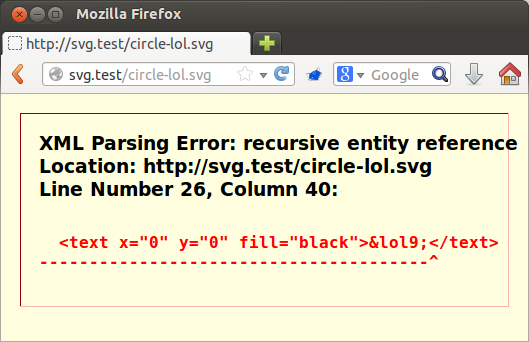
\includegraphics[width=.9\textwidth]{includes/firefox-lol}
\end{subfigure}%
\begin{subfigure}{.5\textwidth}
  \centering
  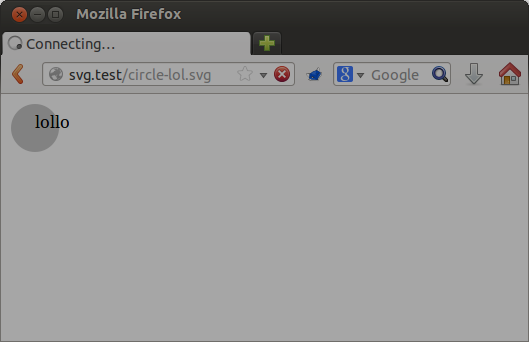
\includegraphics[width=.9\textwidth]{includes/firefox-lol2}
\end{subfigure}
\end{figure}
\end{frame}

\begin{frame}[fragile]{Attacking the DOM}{Innocent HTML}
  \lstinputlisting[style=small1HTML,linebackgroundcolor={\btLstHL<1>{8-11}}]{includes/dom-victim.html}
\end{frame}

\begin{frame}[fragile]{Attacking the DOM}{As rendered}
  \hfill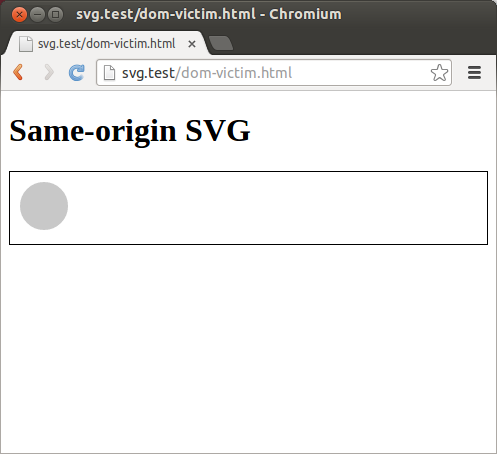
\includegraphics[height=5cm]{includes/dom-normal}\hspace*{\fill}
\end{frame}

\begin{frame}[fragile]{Attacking the DOM}{Malicious SVG}
  \lstinputlisting[style=small2XML,linebackgroundcolor={\btLstHL<1>{8-15}}]{includes/dom-attacker.svg}  
\end{frame}

\begin{frame}[fragile]{Attacking the DOM}{Results}
  \hfill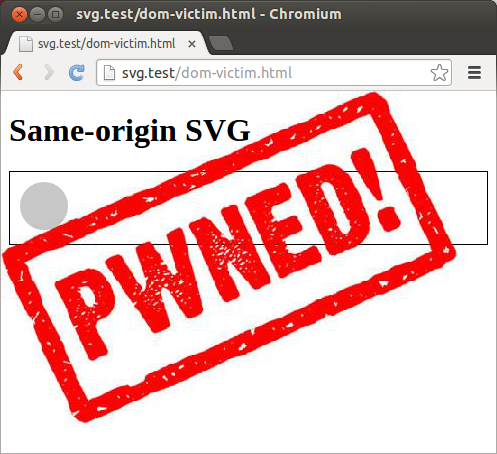
\includegraphics[height=5cm]{includes/dom-attack}\hspace*{\fill}
\end{frame}

\begin{frame}[fragile]{XSS}{Code}
  \lstinputlisting[style=small1XML,linebackgroundcolor={\btLstHL<1>{15}}]{includes/circle-xss.svg.php}  
\end{frame}

\begin{frame}[fragile]{XSS}{Results}
\begin{figure}
\centering
\begin{subfigure}{.5\textwidth}
  \centering
  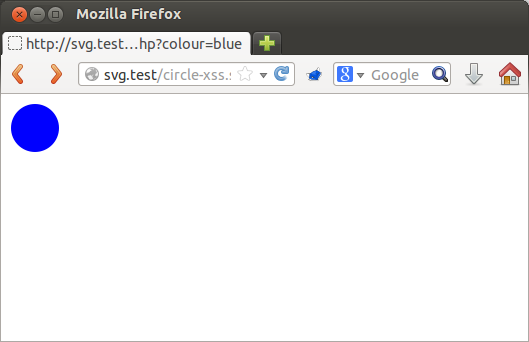
\includegraphics[width=.9\textwidth,valign=t]{includes/xss-normal}
  \caption{\texttt{http://svg.test/circle-xss.svg.php\-?colour=blue}}
\end{subfigure}%
\begin{subfigure}{.5\textwidth}
  \centering
  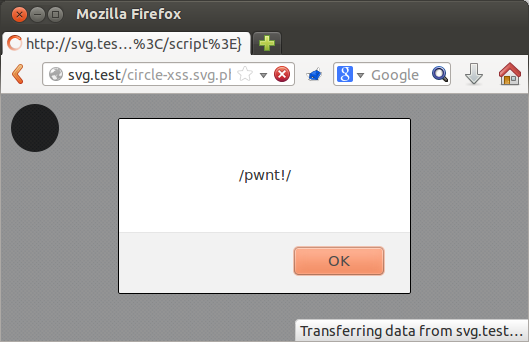
\includegraphics[width=.9\textwidth,valign=t]{includes/xss-attack}
  \caption{\texttt{http://svg.test/circle-xss.svg.php\- ?colour="/><script>alert(/pwnt!/);\-</script>}}
\end{subfigure}
\end{figure}
\end{frame}

\subsection{Security model}

\begin{frame}[fragile]{Security model}
  \begin{itemize}
    \item SVG loaded as static images are treated like other image formats:
    \begin{itemize}
      \item External resources (stylesheets, scripts, other images, etc.) are not loaded.
      \item Scripts are never executed.
      \item Internal stylesheets and \texttt{data} URIs are allowed.
    \end{itemize}
    \item SVG loaded as nested documents are treated just like HTML:
    \begin{itemize}
      \item External resources are loaded.
      \item Scripts are executed.
      \item Same-Origin Policy applies.
      \item Sandboxed iframes disable script execution
      \item Browsers must never load a document as a child of itself.
    \end{itemize}
    \item In-line SVG is just tags, but security rules apply to any external resources used by in-line SVG.
  \end{itemize}
\end{frame}
  
  
\subsection{Security model violations}

\begin{frame}[fragile]{Internet Explorer always loads external CSS}{Source}
\begin{figure}
\centering
\begin{subfigure}{.5\textwidth}
  \centering
  \lstinputlisting[style=small2HTML,linebackgroundcolor={\btLstHL<1>{9}}]{includes/external-css.html}  
\end{subfigure}%
\begin{subfigure}{.5\textwidth}
  \centering
  \lstinputlisting[style=small2XML,linebackgroundcolor={\btLstHL<1>{3-4}}]{includes/circle-css-external.svg}
\end{subfigure}
\end{figure}
\end{frame}

\begin{frame}[fragile]{Internet Explorer always loads external CSS}{Results}
\begin{figure}
\centering
\begin{subfigure}{.5\textwidth}
  \centering
  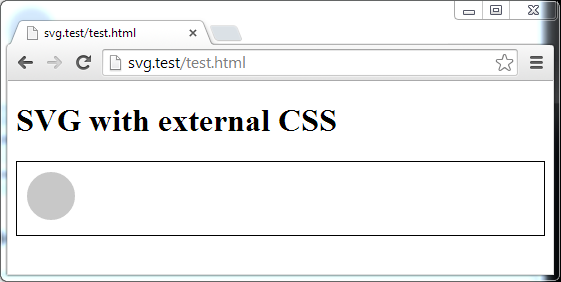
\includegraphics[width=.9\textwidth]{includes/chrome-external-css}
  \caption{Chrome}
\end{subfigure}%
\begin{subfigure}{.5\textwidth}
  \centering
  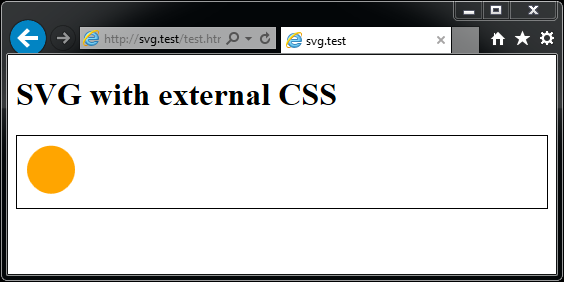
\includegraphics[width=.9\textwidth]{includes/ie-external-css}
  \caption{Internet Explorer}
\end{subfigure}
\end{figure}
CSP \emph{does} block external CSS correctly in the 11.0.9879.0 technical preview build.
\end{frame}

\begin{frame}[fragile]{Chrome loads cross-origin CSS}{Source}
\begin{figure}
\centering
\begin{subfigure}{.5\textwidth}
  \centering
  \lstinputlisting[style=small2HTML,linebackgroundcolor={\btLstHL<1>{9}}]{includes/cross-origin-css.html}
\end{subfigure}%
\begin{subfigure}{.5\textwidth}
  \centering
  \lstinputlisting[style=small2XML,linebackgroundcolor={\btLstHL<1>{3-4}}]{includes/circle-css-cross-domain.svg}
\end{subfigure}
\end{figure}
\end{frame}

\begin{frame}[fragile]{Chrome loads cross-origin CSS}{Results}
\begin{figure}
\centering
\begin{subfigure}{.5\textwidth}
  \centering
  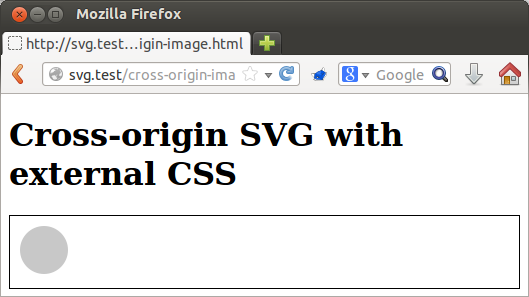
\includegraphics[width=.9\textwidth]{includes/cross-origin-css-firefox}
  \caption{Firefox}
\end{subfigure}%
\begin{subfigure}{.5\textwidth}
  \centering
  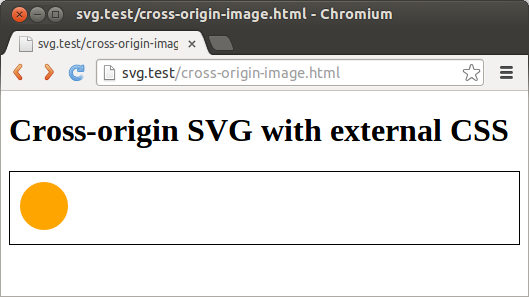
\includegraphics[width=.9\textwidth]{includes/cross-origin-css-chrome}
  \caption{Chrome}
\end{subfigure}
\end{figure}
{\tiny Chrome bug 384527\footnote{\url{https://code.google.com/p/chromium/issues/detail?id=384527}}; fixed in Chromium build 37.0.2054.0, picked up by Apple as CVE-2014-4465\footnote{\url{http://support.apple.com/en-us/HT6596}}}
\end{frame}

\begin{frame}[fragile]{Internet Explorer always loads external images}{Source}
\begin{figure}
\centering
\begin{subfigure}{.5\textwidth}
  \centering
  \lstinputlisting[style=small2HTML,linebackgroundcolor={\btLstHL<1>{9-10}}]{includes/img-svg-image.html}
\end{subfigure}%
\begin{subfigure}{.5\textwidth}
  \centering
  \lstinputlisting[style=small2XML,linebackgroundcolor={\btLstHL<1>{15-16}}]{includes/recurse1.svg}
\end{subfigure}
\end{figure}
\end{frame}

\begin{frame}[fragile]{Internet Explorer always loads external images}{Results}
\begin{figure}
\centering
\begin{subfigure}{.5\textwidth}
  \centering
  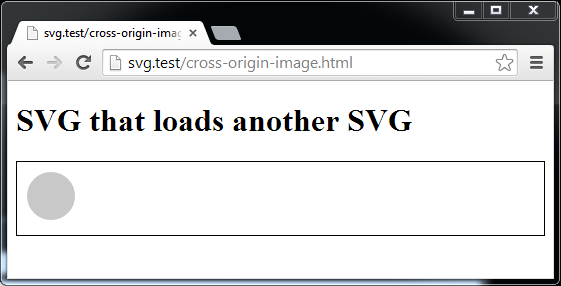
\includegraphics[width=.9\textwidth]{includes/img-svg-image-chrome}
  \caption{Chrome}
\end{subfigure}%
\begin{subfigure}{.5\textwidth}
  \centering
  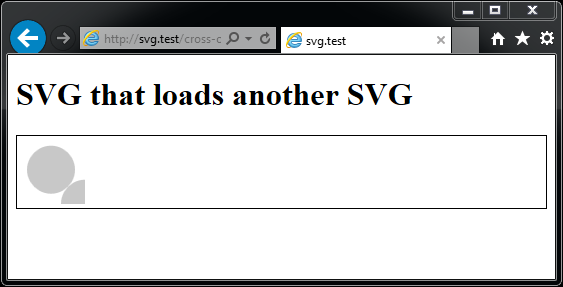
\includegraphics[width=.9\textwidth]{includes/img-svg-image-ie}
  \caption{Internet Explorer}
\end{subfigure}
\end{figure}
{\tiny Reported to Microsoft; ``Not a security bug''.}\\
CSP \emph{does} block external images correctly in the 11.0.9879.0 technical preview build.
\end{frame}

\begin{frame}[fragile]{Recursion}{We get SVGnal. Main SVGeen turn on.}
\begin{figure}
  \centering
  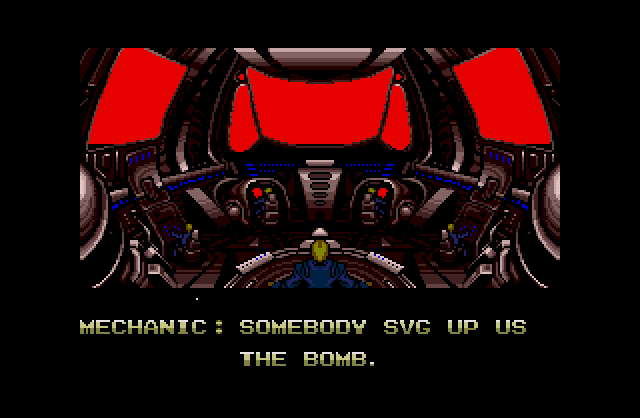
\includegraphics[height=5cm]{includes/somebody-svg-up-us-the-bomb}
\end{figure}
\end{frame}

\begin{frame}[fragile]{Recursion}
  \begin{itemize}
    \item Browsers' checks for recursive documents are based on the URI.  So as long as the URI changes at every iteration, we can make a recursive document.
    \item The query string is part of the URI, but is ignored by HTTP file servers.
    \item To change the query string at every iteration, we need scripting.
    \item We can't use \texttt{svg:image} because that doesn't run scripts, so we use \texttt{html:object} inside \texttt{svg:foreignObject}.
    \item Internet Explorer doesn't render \texttt{svg:foreignObject}\footnote{\url{http://msdn.microsoft.com/en-us/library/hh834675(v=vs.85).aspx}}, but IE does run scripts and load external documents inside it!
  \end{itemize}
\end{frame}

\begin{frame}[fragile]{Recursion}{Code}
  \lstinputlisting[style=small2HTML,linebackgroundcolor={\btLstHL<1>{8-15,18-19}}]{includes/recursive-foreignobject.svg}
\end{frame}

\begin{frame}[fragile]{Recursion}{As rendered in Firefox}
\begin{figure}
  \centering
  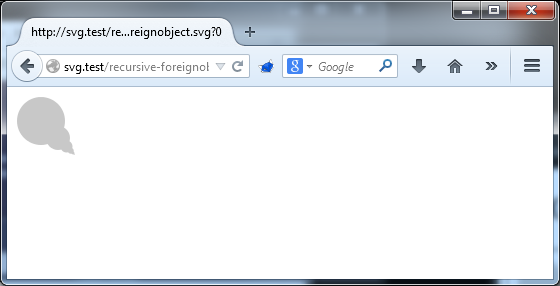
\includegraphics[height=5cm]{includes/recurse-firefox}
\end{figure}
Firefox stops at 10 iterations.
\end{frame}

\begin{frame}[fragile]{Recursion}{As rendered in Chrome}
\begin{figure}
  \centering
  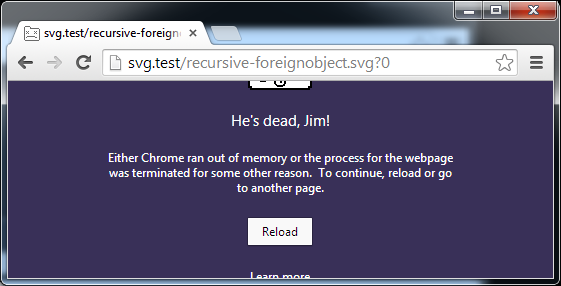
\includegraphics[height=5cm]{includes/recurse-chrome}
\end{figure}
Chrome bug 383180\footnote{\url{https://code.google.com/p/chromium/issues/detail?id=383180}}: tab crash after \textasciitilde 241 iterations.
\end{frame}

\begin{frame}[fragile]{Recursion}{As rendered in Internet Explorer}
\begin{figure}
  \centering
  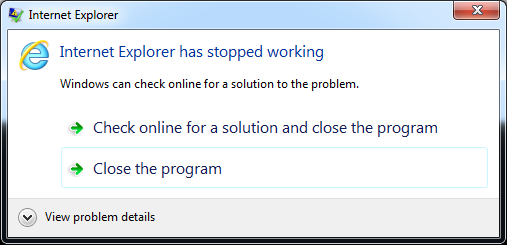
\includegraphics[height=5cm]{includes/recurse-ie}
\end{figure}
Tab crash in IE 11 and 12 DC1 after >4000 iterations.

{\tiny Reported to Microsoft; ``Not a security bug''.}
\end{frame}

\begin{frame}[fragile]{Recursion}{IE and \texttt{image}}
  \lstinputlisting[style=small2js,linebackgroundcolor={\btLstHL<1>{6,16}}]{includes/recursive-image.js}
\end{frame}

\begin{frame}[fragile]{Recursion}{As rendered in IE}
\begin{figure}
  \centering
  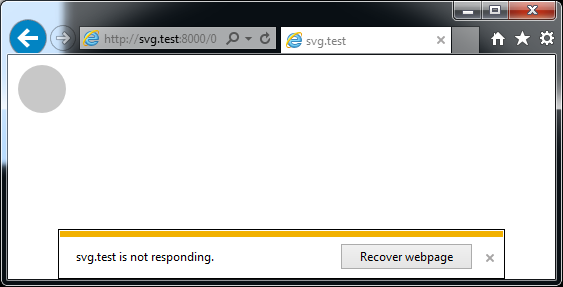
\includegraphics[height=4.5cm]{includes/recurse-ie-image}
\end{figure}
IE 11 and 12 DC1 run >250,000 iterations before crashing, which takes a while.

{\tiny Reported to Microsoft; ``Not a security bug''.}
\end{frame}

\subsection{CSP Violations}

\begin{frame}[fragile]{Chrome \texttt{style-src} violation}
When an SVG with in-line CSS is loaded with \texttt{style-src 'self'} from a static image context, the CSS is applied contrary to the CSP\footnote{\url{https://code.google.com/p/chromium/issues/detail?id=378500}}.
\begin{figure}
\centering
\begin{subfigure}{.5\textwidth}
  \centering
  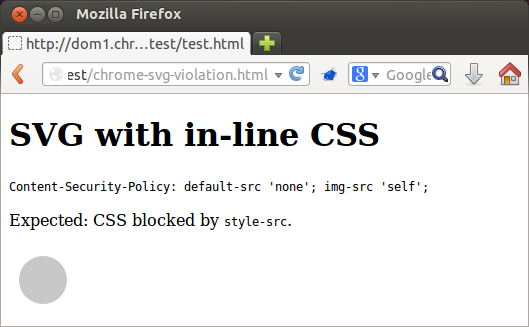
\includegraphics[width=.9\textwidth]{includes/firefox-csp-correct}
  \caption{Firefox}
\end{subfigure}%
\begin{subfigure}{.5\textwidth}
  \centering
  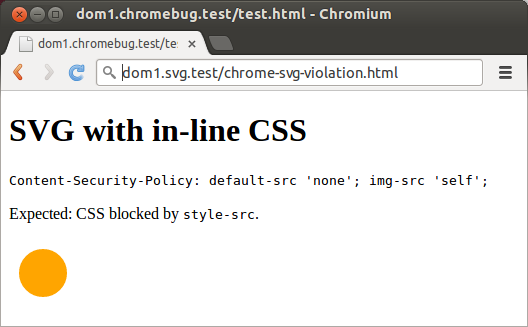
\includegraphics[width=.9\textwidth]{includes/chrome-csp-violation}
  \caption{Chrome}
\end{subfigure}
\end{figure}
{\tiny Chrome bug 378500.  No action since 30 May.}
\end{frame}

\begin{frame}[fragile]{Chrome \texttt{frame-src} vs. \texttt{object-src}}{\texttt{object-src 'self'; frame-src 'none'}}
  Either \texttt{frame-src} and \texttt{object-src} apply to nested browsing contexts, depending on the tag used to open the context.  Chrome applies {\em both} \texttt{object-src} and \texttt{frame-src} to HTML \texttt{object} and \texttt{embed} tags, rather than only \texttt{object-src}\footnote{\url{https://code.google.com/p/chromium/issues/detail?id=400840}}.
\begin{figure}
\centering
\begin{subfigure}{.5\textwidth}
  \centering
  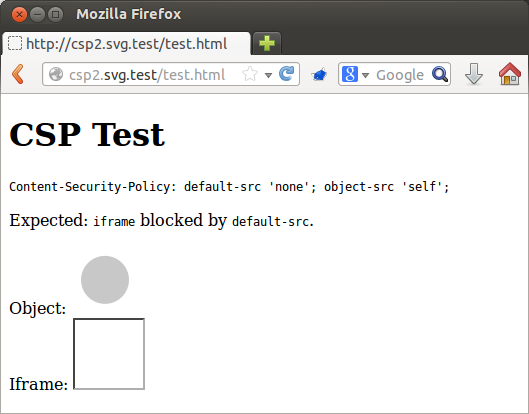
\includegraphics[width=.9\textwidth]{includes/firefox-csp-object}
  \caption{Firefox}
\end{subfigure}%
\begin{subfigure}{.5\textwidth}
  \centering
  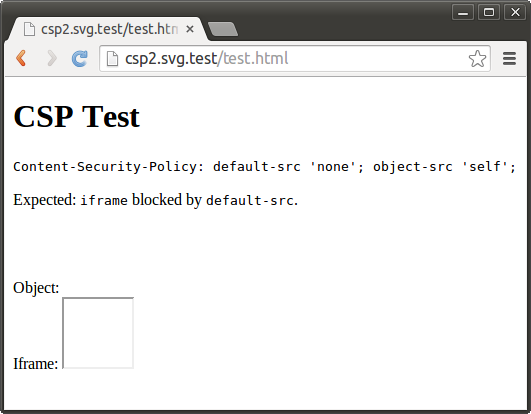
\includegraphics[width=.9\textwidth]{includes/chrome-csp-object}
  \caption{Chrome}
\end{subfigure}
\end{figure}
\end{frame}

\begin{frame}[fragile]{\texttt{frame-src} vs. \texttt{object-src}}{\texttt{object-src 'none'; frame-src 'self'}}
  Either \texttt{frame-src} and \texttt{object-src} apply to nested browsing contexts, depending on the tag used to open the context.  Chrome applies {\em both} \texttt{object-src} and \texttt{frame-src} to HTML \texttt{object} and \texttt{embed} tags, rather than only \texttt{object-src}\footnote{\url{https://code.google.com/p/chromium/issues/detail?id=400840}}.
\begin{figure}
\centering
\begin{subfigure}{.5\textwidth}
  \centering
  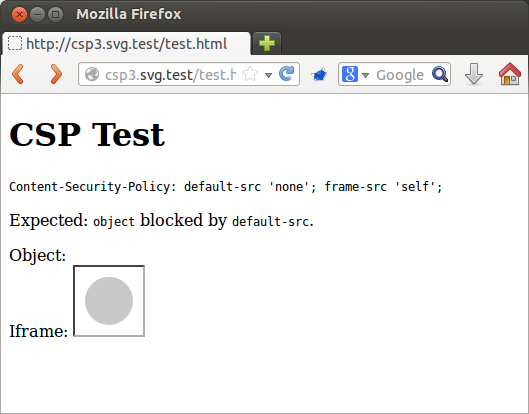
\includegraphics[width=.9\textwidth]{includes/firefox-csp-frame}
  \caption{Firefox}
\end{subfigure}%
\begin{subfigure}{.5\textwidth}
  \centering
  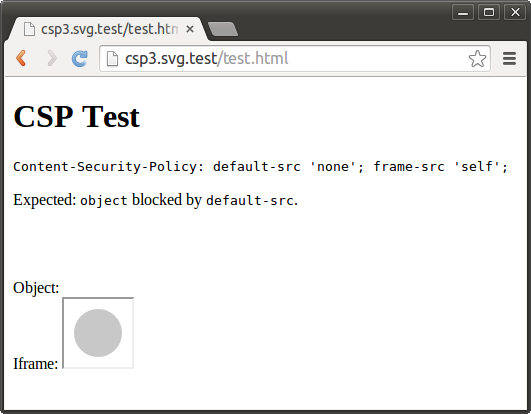
\includegraphics[width=.9\textwidth]{includes/chrome-csp-frame}
  \caption{Chrome}
\end{subfigure}
\end{figure}
\end{frame}

\begin{frame}[fragile]{\texttt{frame-src} vs. \texttt{object-src}}{\texttt{object-src 'self'; frame-src 'self'}}
  Either \texttt{frame-src} and \texttt{object-src} apply to nested browsing contexts, depending on the tag used to open the context.  Chrome applies {\em both} \texttt{object-src} and \texttt{frame-src} to HTML \texttt{object} and \texttt{embed} tags, rather than only \texttt{object-src}\footnote{\url{https://code.google.com/p/chromium/issues/detail?id=400840}}.
\begin{figure}
\centering
\begin{subfigure}{.5\textwidth}
  \centering
  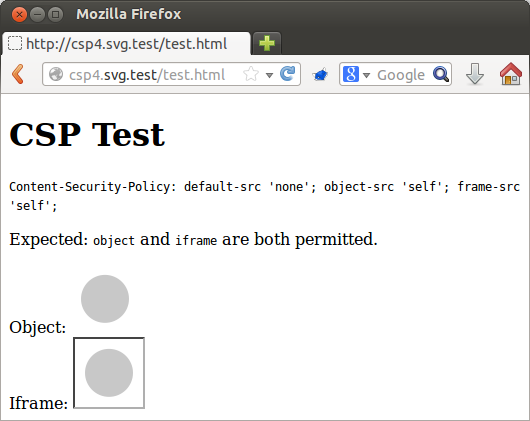
\includegraphics[width=.9\textwidth]{includes/firefox-csp-object-frame}
  \caption{Firefox}
\end{subfigure}%
\begin{subfigure}{.5\textwidth}
  \centering
  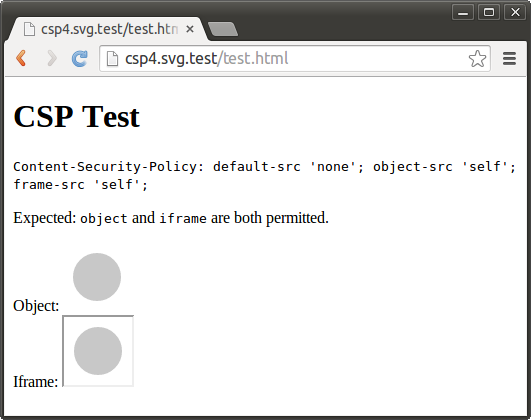
\includegraphics[width=.9\textwidth]{includes/chrome-csp-object-frame}
  \caption{Chrome}
\end{subfigure}
\end{figure}
\end{frame}

\begin{frame}[fragile]{Sandboxed \texttt{iframe}s in Chrome}
  Chrome ignores \texttt{'self'} on all CSP directives in sandboxed \texttt{iframe}s\footnote{\url{https://code.google.com/p/chromium/issues/detail?id=443444}}.
\begin{figure}
\centering
\begin{subfigure}{.5\textwidth}
  \centering
  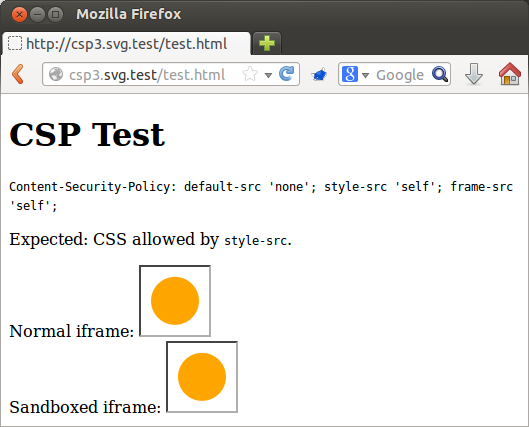
\includegraphics[width=.9\textwidth]{includes/firefox-sandboxed-iframe}
  \caption{Firefox}
\end{subfigure}%
\begin{subfigure}{.5\textwidth}
  \centering
  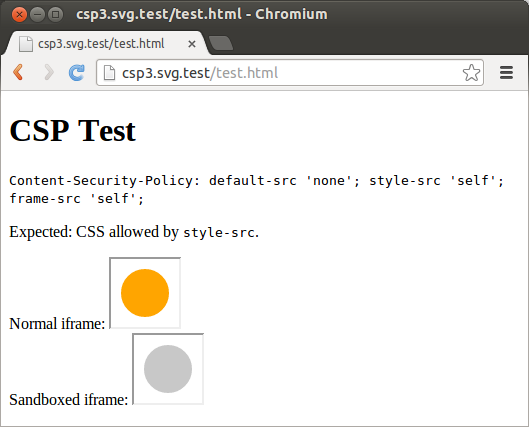
\includegraphics[width=.9\textwidth]{includes/chrome-sandboxed-iframe}
  \caption{Chrome}
\end{subfigure}
\end{figure}
Work-around: list the origin explicitly in CSP rather than relying on \texttt{'self';}
\end{frame}

\begin{frame}[fragile]{Other issues}
  \begin{itemize}
    \item Firefox did not properly apply CSP to sandboxed iframes prior to version 28.0.  This appears to have been due to wider problems with sandboxed iframes.
    \item Neither Chrome nor Firefox render foreignObjects in in-line SVG.
    %\item Both Chrome\footnote{\url{https://code.google.com/p/chromium/issues/detail?id=378500}} and Firefox\footnote{\url{https://bugzilla.mozilla.org/show_bug.cgi?id=1018310}} display in-line SVG even under the CSP \texttt{default-src 'none';}.  The position of the browser authors is that in-line SVG is ``just tags'' and not subject to CSP.  I'm not sure that I agree; conceptually, there isn't much difference between an in-line SVG and an SVG encoded as a \texttt{data:} URI to an \texttt{object} tag, which can be restricted using CSP.
    %\item \texttt{style-src} didn't prevent Chrome from incorrectly loading cross-origin stylesheets from static image SVGs\footnote{\url{https://code.google.com/p/chromium/issues/detail?id=378500}}.
  \end{itemize}
\end{frame}

\begin{frame}[fragile]{SVG Security Test Suite}
  \begin{columns}[c]
    \begin{column}[c]{.5\textwidth}
      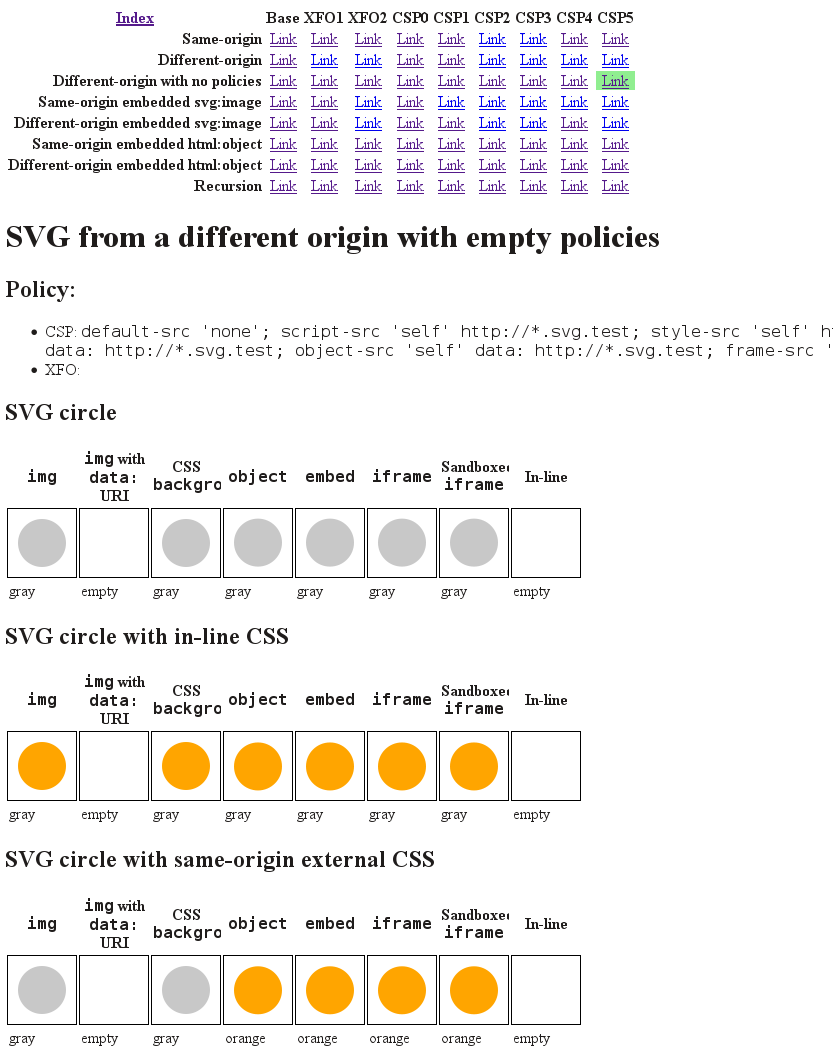
\includegraphics[height=7.5cm]{images/test-suite}
    \end{column}
    \begin{column}[c]{.5\textwidth}
      \begin{itemize}
        \item \url{https://github.com/rdegraaf/SVG_Security_Test_Suite}
        \item Loads different SVGs with internal and external scripts, styles, embedded images, and embedded objects in eight different ways under various XFO and CSP settings.
        \item Just serve it, load it, and look for discrepancies.
      \end{itemize}
    \end{column}
  \end{columns}
\end{frame}

\section{Conclusion}

\begin{frame}[fragile]{Lessons to be learned}
  \begin{itemize}
    \item Treat SVG like you would HTML, not like you would PNG.
    \item Never load untrusted SVG as an object or iframe from the same origin as trusted content.
    \item Major browsers still have issues correctly enforcing web security rules.
    \item CSP is your friend.  Use it.  Even if you can't use it right away, design new code to be CSP-compatible.
  \end{itemize}
\end{frame}

\begin{frame}[fragile]{Future work}
  \begin{itemize}
    \item Mobile browsers
    \item Different CSPs on HTML and embedded SVG
    \item CSP 2.0
    \item SVG 2.0: \texttt{iframe} and \texttt{canvas} and other fun stuff?
    \item SVG's \texttt{use} element and anything else that takes a URI argument
    \item IE12's CSP implementation
  \end{itemize}
\end{frame}

\begin{frame}[fragile]{More information}
  \begin{itemize}
    \item SVG 1.1: \url{http://www.w3.org/TR/SVG/single-page.html}, \url{https://developer.mozilla.org/en-US/docs/Web/SVG}
    \item CSP 1.0: \url{http://www.w3.org/TR/CSP/}, \url{https://developer.mozilla.org/en-US/docs/Web/Security/CSP}, \url{https://www.isecpartners.com/media/106598/csp_best_practices.pdf}
    \item HTML 5: \url{http://www.w3.org/TR/html5/Overview.html}
    \item SVG as a static image: \url{https://developer.mozilla.org/en-US/docs/Web/SVG/SVG_as_an_Image}
    \item Integrating SVG with other stuff: \url{http://www.w3.org/TR/2014/WD-svg-integration-20140417/}
  \end{itemize}
\end{frame}

\begin{frame}[fragile]
  \begin{center}
    \Huge \color{isecdarkgray}\sc Questions? \\
    \small \sc \href{https://www.isecpartners.com}{https://www.isecpartners.com}\\
    \small \sc \href{http://isecpartners.github.io}{http://isecpartners.github.io}
  \end{center}
\end{frame}


\end{document}


